\chapter{2023/10/9}\label{20231009}

\section{2023 Nobel Prize}\label{nobel-prize}

\subsection*{(1) The Nobel Prize in Physics
2023}\label{the-nobel-prize-in-physics-2023}

The Royal Swedish Academy of Sciences has decided to award the Nobel
Prize in Physics 2023 to:

\begin{itemize}
\tightlist{}
\item
  \textbf{Pierre Agostini} (The Ohio State University, Columbus, USA)
\item
  \textbf{Ferenc Krausz} (Max Planck Institute of Quantum Optics,
  Garching and Ludwig-Maximilians-Universität München, Germany)
\item
  \textbf{Anne L'Huillier} (Lund University, Sweden)
\end{itemize}

for \textbf{experimental methods that generate attosecond pulses of
light for the study of electron dynamics in matter}
(产生阿秒光脉冲用于研究物质中电子动力学的实验方法).
\[1 \ \mathrm{attosecond \ (as)} = 10^{-18} \mathrm{s}.\]

We can look at the scale of a hydrogen atom:
\[r \approx 5.3 \times 10^{-10} \ \mathrm{m},\]
\[v \approx 2.2 \times 10^{-6} \ \mathrm{m/s},\]
\[T = {2 \pi r \over v} = 1.52 \times 10^{-16} \ \mathrm{s} = 152 \ \mathrm{as}.\]

Another prize related: The Nobel Prize in Chemistry 1999 was awarded to
Ahmed H. Zewail ``for his studies of the transition states of chemical
reactions using femtosecond spectroscopy''
(利用飞秒光谱法对化学反应过渡态的研究).
\[1 \ \mathrm{femtosecond \ (fs)} = 10^{-15} \mathrm{s}.\]

\subsection*{(2) The Nobel Prize in Chemistry
2023}\label{the-nobel-prize-in-chemistry-2023}

The Royal Swedish Academy of Sciences has decided to award the Nobel
Prize in Chemistry 2023 to

\begin{itemize}
\tightlist{}
\item
  \textbf{Moungi G. Bawendi} Massachusetts Institute of Technology
  (MIT), Cambridge, MA, USA
\item
  \textbf{Louis E. Brus} Columbia University, New York, NY, USA
\item
  \textbf{Alexei I. Ekimov} Nanocrystals Technology Inc., New York, NY,
  USA
\end{itemize}

for \textbf{the discovery and synthesis of quantum dots}.

Confinement (限域效应)

\subsection*{(3) The Nobel Prize in Physiology or Medicine
2023}\label{the-nobel-prize-in-physiology-or-medicine-2023}

The Nobel Assembly at Karolinska Institutet has today decided to award
the 2023 Nobel Prize in Physiology or Medicine jointly to

\begin{itemize}
\tightlist{}
\item
  \textbf{Katalin Karikó}
\item
  \textbf{Drew Weissman}
\end{itemize}

for \textbf{their discoveries concerning nucleoside base modifications
that enabled the development of effective mRNA vaccines against
COVID-19}.

\section{Nondimensionalization
无量纲化}\label{nondimensionalization-ux65e0ux91cfux7eb2ux5316}

Advantages:
\begin{itemize}
\tightlist{}
\item Not restricted by unit systems
\item Guaranteed by similarity
\item Able to be applied widely
\end{itemize}

Take the nondimensionalization of the Navier-Stokes equations
纳维-斯托克斯方程:
\[ \underbrace{\partial \boldsymbol v \over \partial t}_{\text{Euler acceleration}} +\underbrace{(\boldsymbol v \cdot \nabla) \boldsymbol v}_{\text{Advective acceleration (non-linear)}} = -{1 \over \rho} \nabla p + \nu \nabla^2 \boldsymbol v\]

\begin{enumerate}
\def\labelenumi{\arabic{enumi}.}
\item
  Choose characteristic values:

  \begin{itemize}
\tightlist{}
  \item
    characteristic velocity 特征速度 \(V_0\)
  \item
    characteristic length 特征尺度 \(L_0\)
  \end{itemize}

  \begin{quote}
  作业:什么叫数量级 (order of magnitude)
  \end{quote}

  We can then use the values above to express the following:

  \begin{itemize}
\tightlist{}
  \item
    characteristic time 特征时间 \(T_0 = \dfrac{L_0}{V_0}\)
  \item
    characteristic pressure 特征压强 (temporarily unknown)
  \end{itemize}
\item
  Mark \textbf{dimensionless (or non-dimensional) values} with an
  asterisk (*) (无量纲的量用*作区分).
\item
  Replace the physical quantities in the original equation with
  dimensionless values.
\end{enumerate}

In this case, \(\boldsymbol v\) shall be replaced by
\(V_0 \cdot \boldsymbol v^*\), \(t\) by \(\dfrac{L_0}{V_0} t^*\),
\(\nabla\) by \(\dfrac{1}{L_0} \nabla^*\).

So the original equation \[{\partial \boldsymbol v \over \partial t} + (\boldsymbol v \cdot \nabla) \boldsymbol v = - {1 \over \rho} \nabla p + \nu \nabla^2 \boldsymbol v\] becomes:
\[ {\partial (V_0 \cdot \boldsymbol v^*) \over \partial \left(\dfrac{L_0}{V_0} t^*\right)} + \left[ (V_0 \cdot \boldsymbol v^*) \cdot \left( \dfrac{1}{L_0} \nabla^* \right) \right] (V_0 \cdot \boldsymbol v^*) = -{1 \over \rho} \left( \dfrac{1}{L_0} \nabla^* \right) p + \nu \cdot \left( \dfrac{1}{L_0} \nabla^* \right)^2 (V_0 \cdot \boldsymbol v^*)\]
\[{V_0^2 \over L_0} \left[{\partial \boldsymbol v^* \over \partial t^*} + (\boldsymbol v^* \cdot \nabla^*) \boldsymbol v^*\right] = - {1 \over \rho L_0}\nabla^* p + {\nu V_0 \over L_0^2} \nabla^{*2} \boldsymbol v^*\]
\[{\partial \boldsymbol v^* \over \partial t^*} + (\boldsymbol v^* \cdot \nabla^*) \boldsymbol v^* = - {1 \over \rho V_0^2}\nabla^* p + {\nu \over V_0 L_0} \nabla^{*2} \boldsymbol v^*.\]

Let \(\displaystyle p^* = {p \over \rho v_0^2}\), which fills the
\textbf{characteristic pressure} gap mentioned above, and Reynolds
number (雷诺数)
\[Re = {V_0L_0 \over \nu} = {\rho V_0L_0 \over \mu} \ (\nu = {\mu \over \rho}),\]
and the equation becomes
\[{\partial \boldsymbol v^* \over \partial t^*} + (\boldsymbol v^* \cdot \nabla^*) \boldsymbol v^* = - \nabla^* p^* + {1 \over Re} \nabla^{*2} \boldsymbol v^*.\]

\begin{quote}
作业:非线性项雷诺数的推导 (?)
\end{quote}

\section{Mass 质量}\label{mass-ux8d28ux91cf}

There are two types of masses:

\begin{itemize}
\tightlist{}
\item
  Inertia mass 惯性质量 \(m_i\) \[\boldsymbol F = m_i \boldsymbol a\]
\item
  Gravitational mass 引力质量 \(m_g\)
  \[\boldsymbol F = {GMm_g \over r^2} \hat{\boldsymbol r} \]
\end{itemize}

According to the equivalence principle (等效原理), it holds that
\[m_i \equiv m_g.\]

\begin{quote}
作业:什么是爱因斯坦的电梯思想实验?局域性指什么?
\end{quote}

There are two forms of the equivalence principle: the \textbf{weak}
equivalence principle (WEP for short) and the \textbf{strong}
equivalence principle.

We know that positive matter meets with WEP. But, does antimatter?

(27 September 2023 on 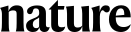
\includegraphics[height=10pt]{assets/Nature.png}: \emph{Observation of the effect of gravity on the motion of antimatter} (\url{https://doi.org/10.1038/s41586-023-06527-1}) and \emph{Free-falling antihydrogen reveals the effect of gravity on antimatter} (\url{https://doi.org/10.1038/d41586-023-02930-w}).)
